%%%%%%%%%%%%%%%%%%%%%%%%%%%%%
%Since : Jan/29/2009
%Update: <Mar/13/2013>
% -*- coding: iso-2022-jp -*-
%%%%%%%%%%%%%%%%%%%%%%%%%%%%%

\chapter{ネットワーク基礎演習1}
\section{目的}

サーバ用途でよく用いられるUnix, Linuxの基本的な操作を学ぶことを目的とする。

\section{Unix, Linux}

UNIXはマルチユーザ(1台のコンピュータを複数の利用者で共有する), マルチプロセス
(複数のプログラムを平行して実行する), ネットワーク機能に優れたオペレーティング
システムである。UNIXはインターネットやLANが普及し始めた頃, これらのネットワークに
接続するコンピュータの標準的なOSとして世界中に普及した。今日でも, ネットワーク上
のさまざまなサービスを提供するサーバ用のコンピュータや, 多くのコンピュータに仕事
を分割して処理するような並列・分散環境ではUNIXが利用されていることが多い。本演習
では, UNIXのクローンOSであるLinuxを用いる。

\section{学科PC室の構成 }

学科PC室にはWindows 用サーバ(com03), Linux用サーバ(cpjsv), レーザープリンタ
(cpjlbp), 演習用webサーバ(cpjweb), 演習用コンピュータ(cpj201--cpj216)が設置されている。演
習用コンピュータにはOSとしてMicrosoft Windows 7 Professional とCent OSが
インストールされている。私達はコンピュータを起動する際に, 使用するOSを選択するこ
とができる。\figref{fig:cpj}にUNIXの利用環境の概要を示す。ユーザ情報や各自のホームディレクト
リ (Windows のマイドキュメントに相当する。Windowsにおけるフォルダを, UNIXではディ
レクトリと呼ぶ)はサーバに一括して保存されている。ユーザ情報はNIS(Network
Information System)という仕組みを使用して, ホームディレクトリはNFS(Network File
System)という仕組みを使用して演習用コンピュータに配信されている。このため, ユー
ザはどのコンピュータにログインしても, 同じ環境で利用することができる。

\begin{figure}[htbp]
\begin{center}
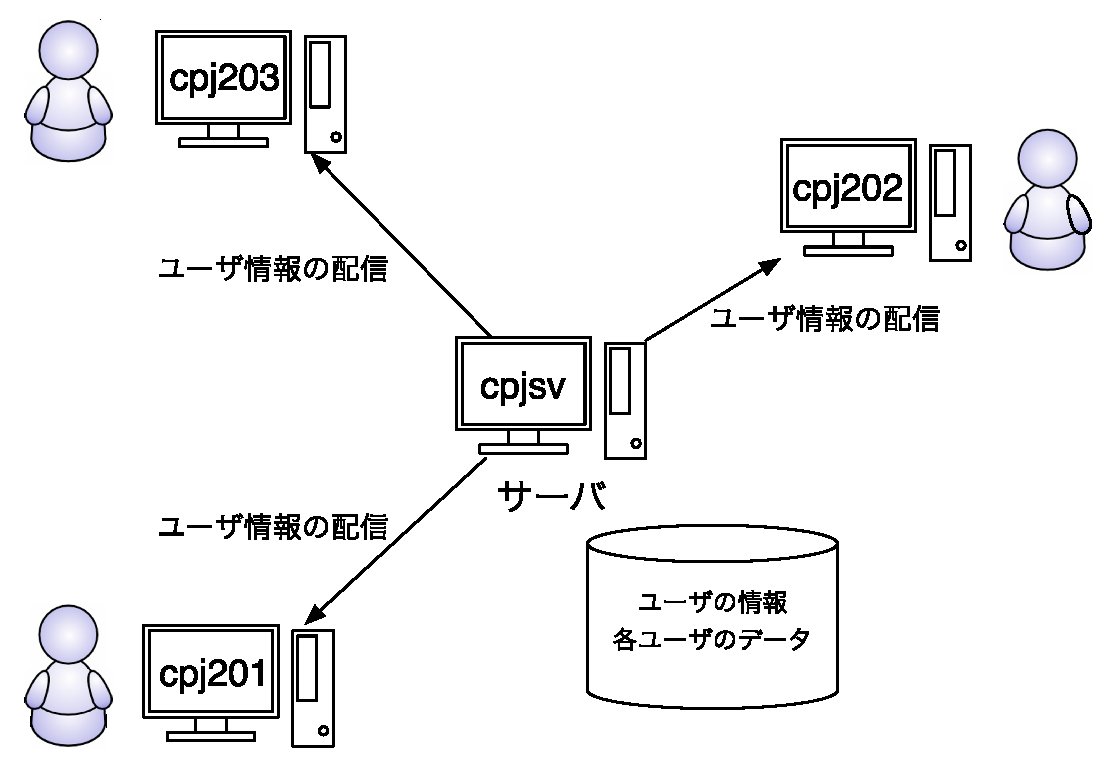
\includegraphics[width=0.8\linewidth]{cpj.eps}
\caption{ユーザの利用環境}
\label{fig:cpj}
\end{center}
\end{figure}

\section{Linuxのディレクトリ構造}
\figref{fig:win-tree}にMicrosoft Windowsのディレクトリ構造の例を示す。ハードディスクは``Cドライ
ブ'', CD-ROMは``Dドライブ''といったように, たいていは1つのディスクに1つのドライブ
名が割当てられている。各々のドライブは木をさかさまにしたような構造をしており, ルー
トフォルダ($\backslash$)を根として, 次々に枝分かれしているように見える。Windows
の場合, このような木がドライブの数だけ存在するようにみえる。\figref{fig:unix-tree}にUNIXのディレク
トリ構造の例を示す。UNIX, Linuxの場合, ディスクが何台あっても, ルートディレクトリ(/)を根
とする1本の木しか存在しない。各々のディスクはどこかのディレクトリに割り付けられる。
ディスク上にあるディレクトリやファイルを参照するためには, それらの位置を特定する
必要がある。このための表記をパス(path)と呼ぶ。例えば, \figref{fig:win-tree}において, Cドライブの
``System''ディレクトリのパスは``C:$\backslash$Windows$\backslash$System''と表記で
きる。Windows ではディレクトリ名を``$\backslash$''でつないでパスを表記する。一方,
UNIXではディレクトリ名を``/''でつないでパスを表記する。例えば, \figref{fig:unix-tree}の``lib''ディ
レクトリのパスは, ``/usr/lib''と表せる。

\begin{figure}[htbp]
\begin{center}
\includegraphics[width=0.7\linewidth]{win-tree.eps}
\caption{Windowsのディレクトリ構造の例}
\label{fig:win-tree}
\end{center}
\end{figure}

\begin{figure}[htbp]
\begin{center}
\includegraphics[width=0.5\linewidth]{unix-tree.eps}
\caption{UNIX, Linuxのディレクトリ構造の例}
\label{fig:unix-tree}
\end{center}
\end{figure}

\section{コンピュータの起動}

\begin{enumerate}
\item モニターの電源スイッチを押して電源をONにする。モニターの前面にはいくつかの
ボタンが並んでいる。このうち, 電源スイッチは右端にある。電源がONであれば,
モニターの前面にあるランプが点灯している。
\item 続いて, コンピュータ本体の電源をONにする。電源スイッチは本体の前面に配置さ
れている。
\item コンピュータの電源が投入されると, ``Press any key to enter the menu''と表
      示される。ここで操作しないまま放置するとWindows7が立ち上がるので、何かキー
      を押す。
\item 次にOS選択画面が表示されるので、上下のカーソルキーを使用して``Cent OS''を選択してEnter
      キーを押す。そうするとLinuxが立ち上がる。
\end{enumerate}

\section{ログイン}

\begin{enumerate}
\item Linuxが起動し終えると\figref{fig:login}のような画面が表示される。ここで、
      その他をクリックする。
\item \figref{fig:passwd}のような画面が表示されるので、ユーザ名を入力する。
      ユーザ名は総合情報センターと同じc-○○○○となっている。入力したらログイン
      をクリックする。
\item 次にパスワード入力画面が現れるのでパスワードを入力する。初めて使う場合、パ
      スワードはユーザ名と同じに設定されている。
\item ログインに成功すると, デスクトップ画面(\figref{fig:desktop})が表示される。ログインに失敗すると, 再
び\figref{fig:login}の画面が表示されるので、もう一度ユーザ名とパスワードを入力する。
\end{enumerate}

\begin{figure}[htbp]
\begin{center}
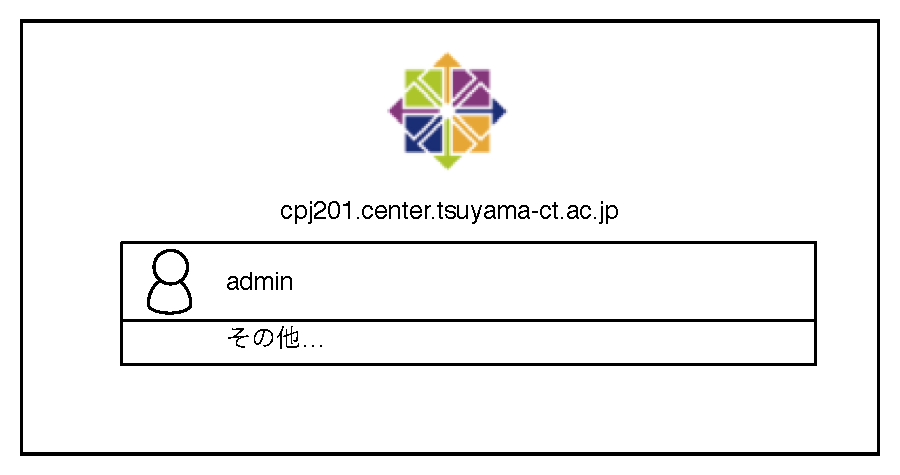
\includegraphics[width=0.3\linewidth]{login.eps}
\caption{ログイン画面}
\label{fig:login}
\end{center}
\end{figure}

\begin{figure}[htbp]
\begin{center}
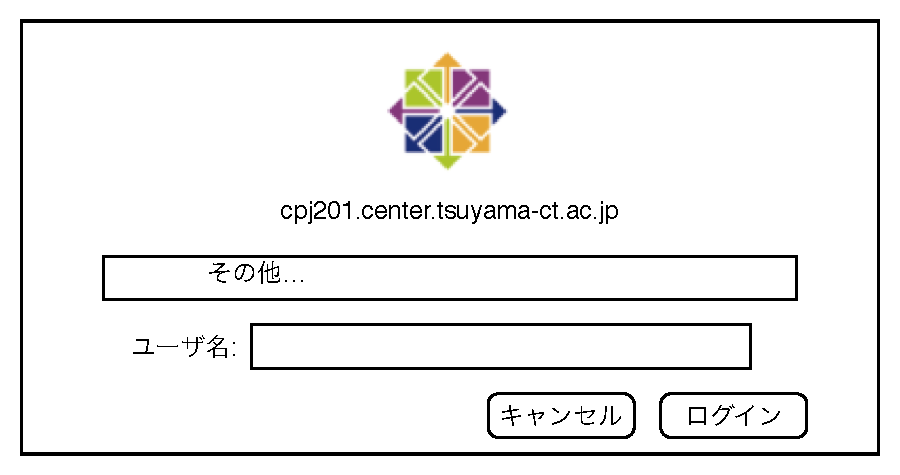
\includegraphics[width=0.3\linewidth]{passwd.eps}
\caption{パスワード入力画面}
\label{fig:passwd}
\end{center}
\end{figure}

\begin{figure}[htbp]
\begin{center}
\includegraphics[width=0.5\linewidth]{desktop.eps}
\caption{デスクトップ画面}
\label{fig:desktop}
\end{center}
\end{figure}

\section{ターミナル(端末エミュレータ )}

Linuxはもともとキーボードで命令を入力して操作することを基本としている。このため,
コンピュータを起動すると, 最初はWindowsのコマンドプロンプトのような画面になる。こ
の画面をコンソールと呼ぶ。しかし, 演習用コンピュータは, Linux が起動すると自動的
にマルチウインドウ・システムが起動するように設定されている。このため, コンソール
を見ることはできない。コンソール画面と同じようにコマンドライン上でキーボードによっ
てコンピュータの操作を行うためのアプリケーションを端末エミュレータ(通称ターミナ
ル)と呼ぶ。本実験では, ターミナルを利用してコンピュータを操作する。

\section{ターミナルの起動 }

\begin{enumerate}
\item \figref{fig:menu}で示すように, デスクトップ画面の左上にあるアプリケーショ
      ンをクリックすると
      この中にあるターミナルのアイコン(\figref{fig:menu}でマウスカーソルがあるところ)をクリックする。
\item \figref{fig:terminal}のようなウインドウ(CentOSに付属のターミナル)が表示される。
\end{enumerate}

\begin{figure}[htbp]
\begin{center}
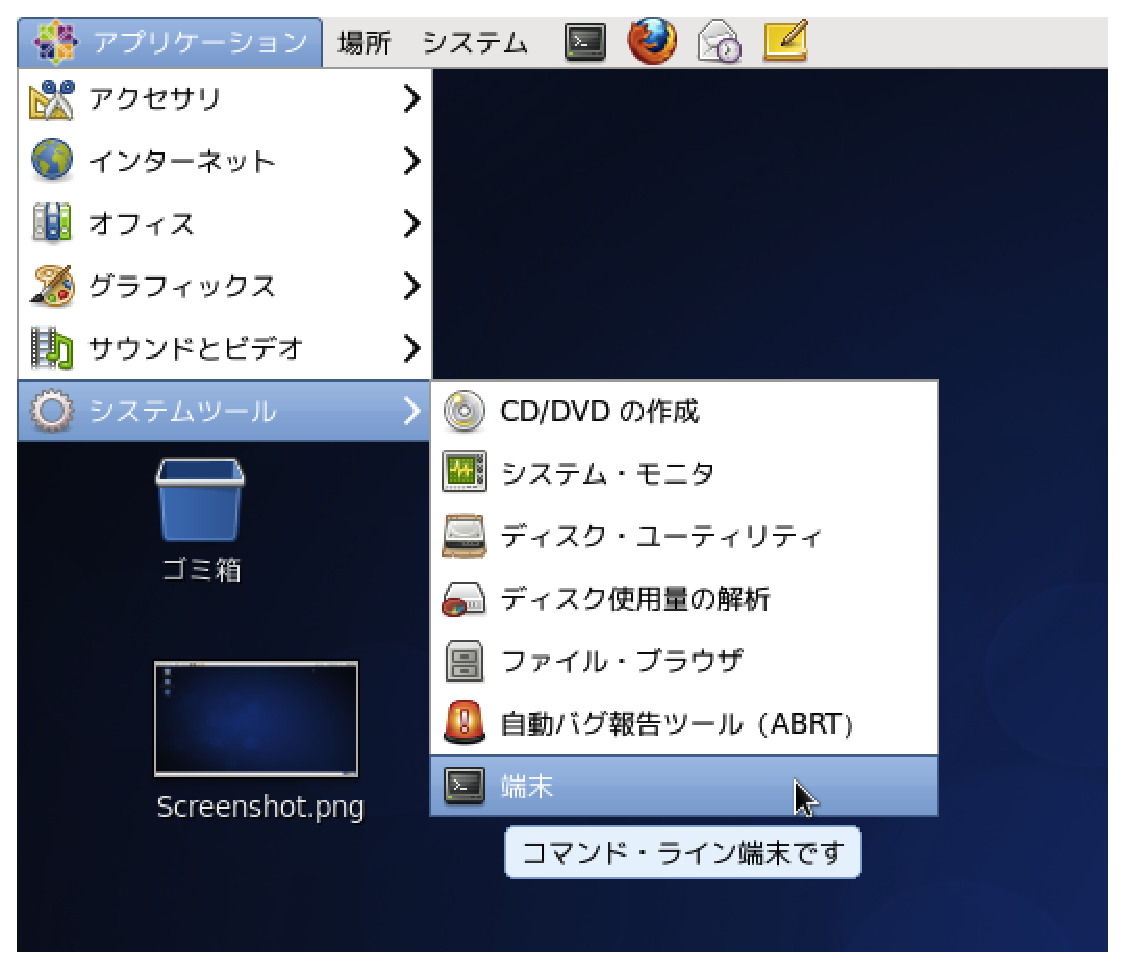
\includegraphics[width=0.5\linewidth]{menu.eps}
\caption{ターミナルのアイコン}
\label{fig:menu}
\end{center}
\end{figure}

\begin{figure}[htbp]
\begin{center}
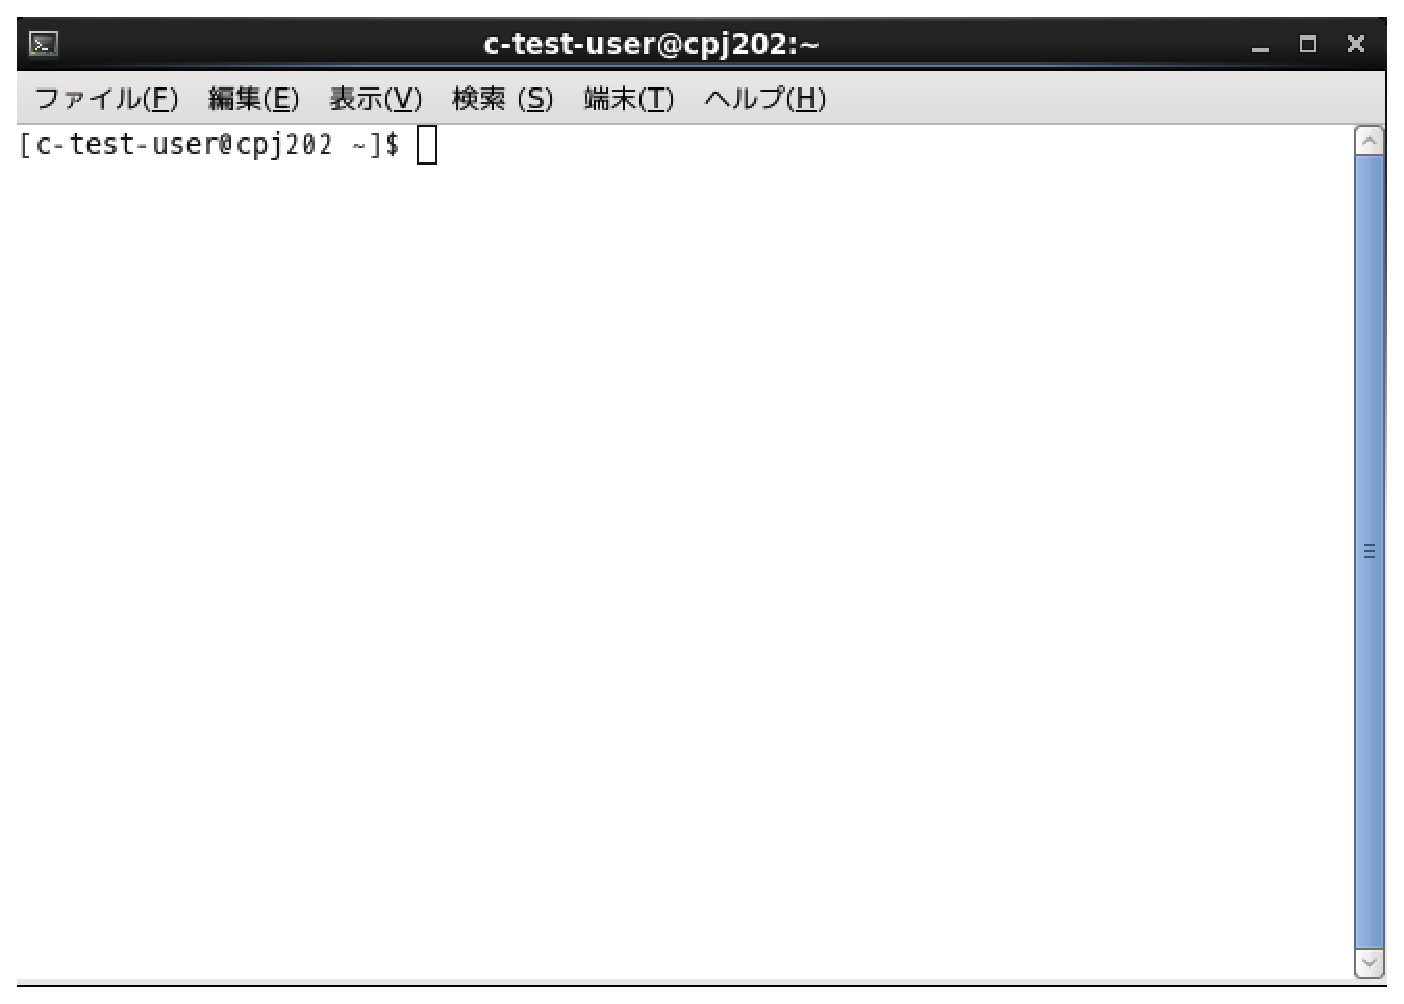
\includegraphics[width=0.5\linewidth]{terminal.eps}
\caption{ターミナルの画面}
\label{fig:terminal}
\end{center}
\end{figure}

\section{コマンドプロンプト }

ターミナルを起動すると, ウインドウの中に\figref{fig:prompt}のようなメッセージが表示され
る。これはユーザにコマンド(命令)の入力を促すメッセージであり, コマンドプロンプ
トという。前半の部分は``ユーザ名@コンピュータ名''となっており, 後半の部分にはカ
レントディレクトリ(ユーザが現在作業しているディレクトリ)が表示される。最後の``\$''
はこの後に命令を入力できることを示している。
コマンドプロンプトはMicrosoft Windowsの``C:$\backslash>$''に相当する。ただし, PC
室のCentOSでは最後の文字が``\$''となる。コマンドプロンプトは, Windowsではアプリケーショ
ンの名称として使用されているが, 一般には命令の入力を促すメッセージのことを指す。

\begin{figure}[htbp]
\begin{center}
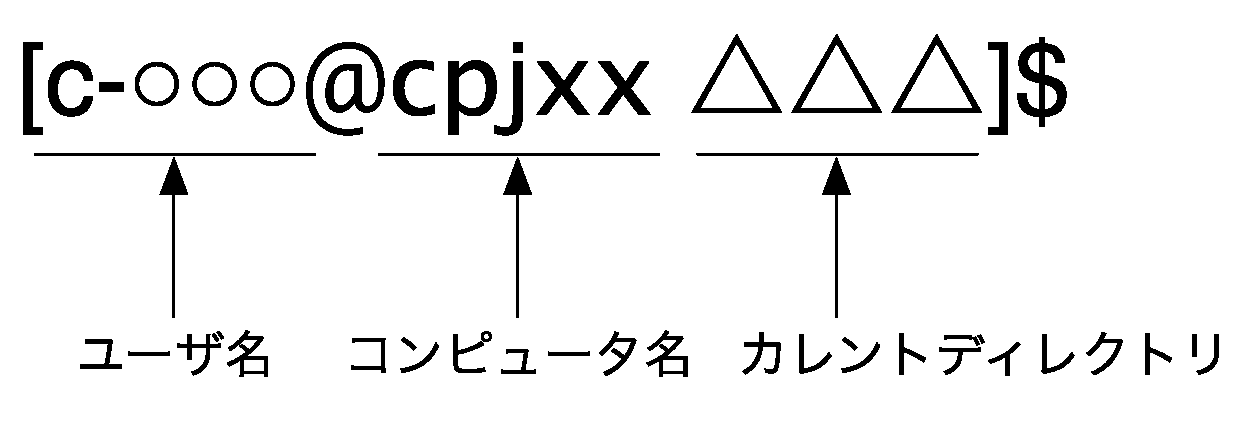
\includegraphics[width=0.5\linewidth]{prompt.eps}
\caption{コマンドプロンプト}
\label{fig:prompt}
\end{center}
\end{figure}

\section{コマンド}
\subsection{pwd}

pwdは``print working directory''の意味で, カレントディレクトリを画面に表示するコマ
ンドである。\figref{fig:pwd}のように, ``pwd''と入力してEnterキーを押すと, カレントディレクト
リの名前(図中では``/homes/c-○○○/△△△'')が表示される。
一般にUNIXでは, ログインした直後にユーザはホームディレクトリにいる。ホームディ
レクトリはユーザ自身のファイルを保存するためのディレクトリで, 例えば
userという名前のユーザなら``/home/user''となっている。
学科PC
室のUNIX環境では, ``c-○○○''というユーザのホームディレクトリは``/homes/c-○○○''
となるように設定されている。

\begin{figure}[htbp]
\begin{center}
\fbox{
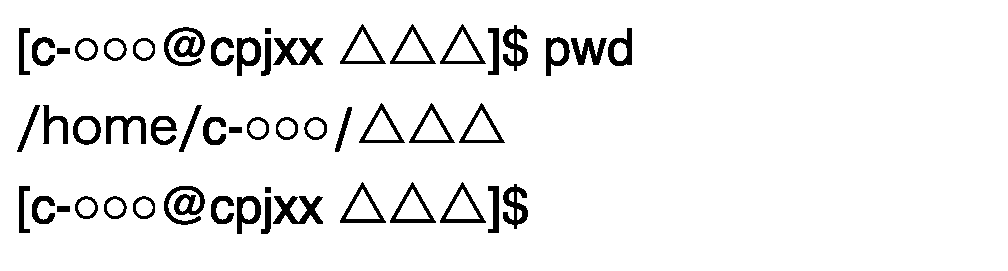
\includegraphics[width=0.5\linewidth]{pwd.eps}
}
\caption{pwdの実行例}
\label{fig:pwd}
\end{center}
\end{figure}

\paragraph{演習}

\begin{enumerate}
\item コマンドプロンプトに続いて, ``pwd''と入力してEnterキーを押す。
\item 現在作業中のディレクトリが表示される。
\end{enumerate}


\subsection{ls}

lsは``list''の意味で, 指定したディレクトリの内容, すなわちそのディレクトリの中に
あるファイルやディレクトリの一覧を表示するコマンドである

\paragraph{演習}
\begin{enumerate}
\item コマンドプロンプトに続いて, ``ls''と入力してEnterキーを押す。
\item 実行するとカレントディレクトリの中にあるディレクトリとファイルの一覧が表示
      される。最後に``/''がついているものは, それがディレクトリであることを意味する。
      最後には再びコマンドプロンプトが表示されることを確認する。
\item コマンドプロンプトに続いて``ls  /usr/lib''と入力して``Enter''キーを押す。これは/usr/lib
      ディレクトリの内容を表示するという意味である。
\item /usr/libディレクトリの中には多数のファイルがあるので, 画面がスクロールしていく。
      最後には再びコマンドプロンプトが表示されることを確認する。
\end{enumerate}

\subsection{cd}

cdは``change directory''の意味で, カレントディレクトリを変更するコマンドである。

\paragraph{演習}
\begin{enumerate}
\item コマンドプロンプトに続いて, ``cd  /homes/data''と入力してEnterキーを押す。
\item cd命令は成功した場合には何も結果が表示されず, コマンドプロ
ンプトに戻る。ただし, プロンプトの中のカレントディレクトリを示す部分が``data''
に変更されていることを確認する。
\item ``pwd''命令を実行して, カレントディレクトリが変更されていることを確認する。
\item 続いて, ``cd  /homes''と入力して, Enterキーを押す。
\item カレントディレクトリが``/homes''に変更されていることを確認する。
\item lsコマンドを使用して, homesディレクトリの内容を表示する。
\item ``cd''を実行し, ホームディレクトリに戻る。そして``pwd''でホームディレクトリである
      ことを確認する。
\end{enumerate}

\subsection{mkdir}

mkdirは``make directory''の意味で, 新しいディレクトリ(Windowsでいうフォルダ)を
作成するコマンドである。mkdirコマンドの例を以下に示す。

\begin{itemize}
\item    mkdir  /homes/data/temp1

        /homes/dataディレクトリの中に, temp1というディレクトリを作成する。

\item    mkdir  temp1

        カレントディレクトリの中に, temp1というディレクトリを作成する。
\end{itemize}

\paragraph{演習}
\begin{enumerate}
\item コマンドプロンプトに続いて``mkdir  data''と入力してEnterキーを押す。これはカレ
      ントディレクトリの中にdataというディレクトリを作成するコマンドである。
\item lsを使用して, 各自のホームディレクトリの中にdataというディレクトリが作成され
      ていることを確認しなさい。
\end{enumerate}

\subsection{cp}

cpは``copy''の意味で, 指定したディレクトリやファイルを別の場所あるいは別の名前
のファイルにコピーする命令である。
  cpの使用方法を以下に示す

\begin{itemize}
\item cp  ファイル1  ファイル2

      ファイル1をファイル2としてコピーする。

\item cp  ファイル   ディレクトリ

       ファイルを指定したディレクトリの中にコピーする。

\item cp -r ディレクトリ1  ディレクトリ2

      ディレクトリ1をディレクトリ2にコピーする。(ディレクトリ2がない場合,
      ディレクトリ2としてコピーする)
\end{itemize}

\paragraph{演習}
\begin{enumerate}
\item コマンドプロンプトに続いて``cp ~ /homes/data/AliceinWonderland.txt ~ /homes/c-○○○''と入力し
てEnter キーを押す(c-○○○は各自のユーザ名に置き換える)。これは, /homes/data
ディレクトリにある``AliceinWonderland.txt''というファイルを/homes/c-○○○ディレクトリの中
にコピーするコマンドである。
\item cpコマンドは成功すると何も表示せず, コマンドプロンプトに戻る。
\item lsコマンドを使用して, ``AliceinWonderland.txt''がコピーされていることを確認する。
\end{enumerate}

\subsection{mv}

mvは``move''の意味で, 指定したディレクトリやファイルを別の場所あるいは別の名前で
移動する命令である。cpと異なる点は, cpの場合は移動元のファイルが残るのに対し, mv
は移動元のファイルは消える点である。

\begin{itemize}
\item mv ファイル1 ファイル2

      ファイル1をファイル2という名前に変更(ファイル1をファイル2というファイルとし
      て移動)

\item mv ファイル ディレクトリ

      ファイルを指定したディレクトリに移動

\item mv ディレクトリ1 ディレクトリ2

      ディレクトリ1をディレクトリ2に移動する。ただし, ディレクトリ2がない場合,
      ディレクトリ1をディレクトリ2として移動する。
\end{itemize}

\paragraph{演習}
\begin{enumerate}
    \item ``mv AliceinWonderland.txt data''と入力してEnterキーを押す
    \item ``cd data''と入力しdataフォルダに移動する
    \item lsを使用してAliceinWonderland.txtが移動されたか確認する。
\end{enumerate}

\subsection{cat}
Unix系のOSでは、OSやソフトの設定や説明はテキストファイルに保存されています。この
ため、Linuxではテキストファイルを読むためのコマンドが沢山入っています。
``cat''もその一つで、ファイルの中身を確認するコマンドです。

\paragraph{演習}
\begin{enumerate}
\item AliceinWonderland.txtがあるディレクトリ(/homes/ユーザ名/data)に移動する。
\item ``cat AliceinWonderland.txt''と入力してEnterキーを押す。
\item 不思議の国のアリス(英語版)が表示されることを確認する。
\end{enumerate}


\subsection{less}
先ほどの``cat''では、ファイルのはじめから順番に表示されるため、1画面に収まりきら
ないテキストの分量でも、最後まで一気に表示されます。このため、長いテキストの場合、
はじめの方が読めず、最後の文章しか読めません。そのような、1画面で収まりきらない
テキストファイルを読むためのコマンドが、``less''です。

\paragraph{演習}
\begin{enumerate}
\item AliceinWonderland.txtがあるディレクトリ(/homes/ユーザ名/data)に移動する。
\item ``less AliceinWonderland.txt''と入力してEnterキーを押す
\item 不思議の国のアリス(英語版)が表示されることを確認する。
\item 上下カーソルキーを押すことで1行表示が前後することを確認する。
\item スペースキーを押すことで、1画面表示が前進することを確認する。
\item qを押し、``less''を終了する。
\end{enumerate}

\subsection{head}
システムのログファイルなどは、ファイルの最初の部分や最後の部分が重要となることが
多く、ファイルの最初や最後の部分だけ確認したい場合が多々ある。``head''は、テキス
トファイルのはじめの数行を表示するコマンドです。

\paragraph{演習}
\begin{enumerate}
\item ``head AliceinWonderland.txt''と入力してEnterキーを押す。
\item 一番上に表示された文字を記録する。
\end{enumerate}

\subsection{tail}
``tail''はテキストファイルの最後の数行を表示するためのコマンドです。

\paragraph{演習}
\begin{enumerate}
\item ``tail AliceinWonderland.txt''と入力してEnterキーを押す。
\item 一番下に表示された文字を記録する。
\end{enumerate}

\subsection{rm}
 rmは``remove''の意味で, 指定されたファイルを削除するコマンドである。

\paragraph{演習}
\begin{enumerate}
\item コマンドプロンプトに続いて``rm  AliceinWonderland.txt''と入力してEnter
      キーを押す。

\item 消去してもよいかをたずねてくる場合は, ``yes''と入力してEnterキーを押す。

\item lsを使用して, AliceinWonderland.txt が削除されていることを確認する。

\end{enumerate}


\section{シャットダウンの仕方}
実験終了の際にはコンピュータをシャットダウンしなければならない。シャットダウンは、
ターミナルに''poweroff''と入力してEnterキーを押せば実行される。

\section{演習問題}

\begin{enumerate}
\item ホームディレクトリ, カレントディレクトリの意味をかけ。

\item 自分のホームディレクトリの場所をpwdで調べ報告せよ。

\item ホームディレクトリに移動するコマンドをかけ。

\item ホームディレクトリにある``ディレクトリ''をlsを用い調べ, そのディレクトリ名を書き出
      せ。

\item AliceinWonderland.txtの最初の行に書かれている文字を書け。
\item AliceinWonderland.txtの最後の行に書かれている文字を書け。

\item ``cat''と``less''の違いを書け。

\end{enumerate}
